\documentclass{beamer}
\usepackage[utf8]{inputenc}
\usepackage{tikz}
\usetikzlibrary{shapes.geometric, arrows}
\tikzstyle{std} = [rectangle, minimum width=7cm, minimum height=0.8cm, text centered, align = center, draw=black, fill=gray!30] 
\tikzstyle{arrow} = [->,>=stealth]
\addtobeamertemplate{navigation symbols}{}{%
    \usebeamerfont{footline}%
    \usebeamercolor[fg]{footline}%
    \hspace{1em}%
    \insertframenumber/\inserttotalframenumber
  }

%Information to be included in the title page:
\title{Competition and Idoelogical Diversity: Historical Evidence from US Newspapers}
\author{Caio Figueiredo}
\institute{Penn State}
\date{2019}
 
\begin{document}
 
\frame{\titlepage}
 
\begin{frame}
  \frametitle{Introduction}
  \begin{itemize}
    \item Objective: Formulate a model of newspaper demand, entry, and political affiliation choice.
  \end{itemize}

\end{frame}

\begin{frame}[t]{Context}
  \begin{itemize}
    \item The year is 1924.
    \item (Most) newspapers openly declare political affiliation.
    \item There is no TV and Radio is at its infancy. Which for us means 
      that the outside option is "No News", simplifying treatment.
  \end{itemize}
\end{frame}

\begin{frame}[t]{Model Sketch}
  \center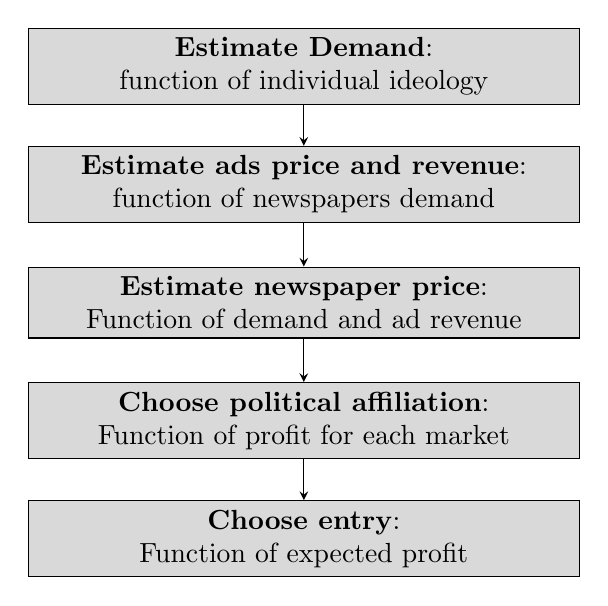
\begin{tikzpicture}[baseline=0, node distance=1.5cm]
    \node (demand) [std, align=center]    
      {\textbf{Estimate Demand}: \\ function of individual ideology};
    \node (ads)    [std, below of=demand] 
      {\textbf{Estimate ads price and revenue}: \\ function of newspapers demand};
    \node (price)  [std, below of=ads]   
      {\textbf{Estimate newspaper price}: \\ Function of demand and ad revenue};
    \node (ideo)   [std, below of=price] 
      {\textbf{Choose political affiliation}: \\ Function of profit for each market};
    \node (entry)  [std, below of=ideo]  
      {\textbf{Choose entry}: \\ Function of expected profit};

    \draw [arrow] (demand) -- (ads);
    \draw [arrow] (ads)    -- (price);
    \draw [arrow] (price)  -- (ideo);
    \draw [arrow] (ideo)   -- (entry);
  \end{tikzpicture}
\end{frame}

\begin{frame}[t]{Data}
  \begin{itemize}
    \item For the supply side (Entry and affiliation), data on the number,
      affiliations, and circulation prices of individual newspaper are used.
      \subitem Collected from newspaper directories
    \item For the demand side, data on circulation per town and newspaper
      is used.
      \subitem Collect from 1924 circulation report.
    \item Supplementary datasets on newspaper revenue and costs, alongside readership
      surveys, are used to calibrate the model
  \end{itemize}
\end{frame}


\end{document}

